\begin{figure}[h]
\centering
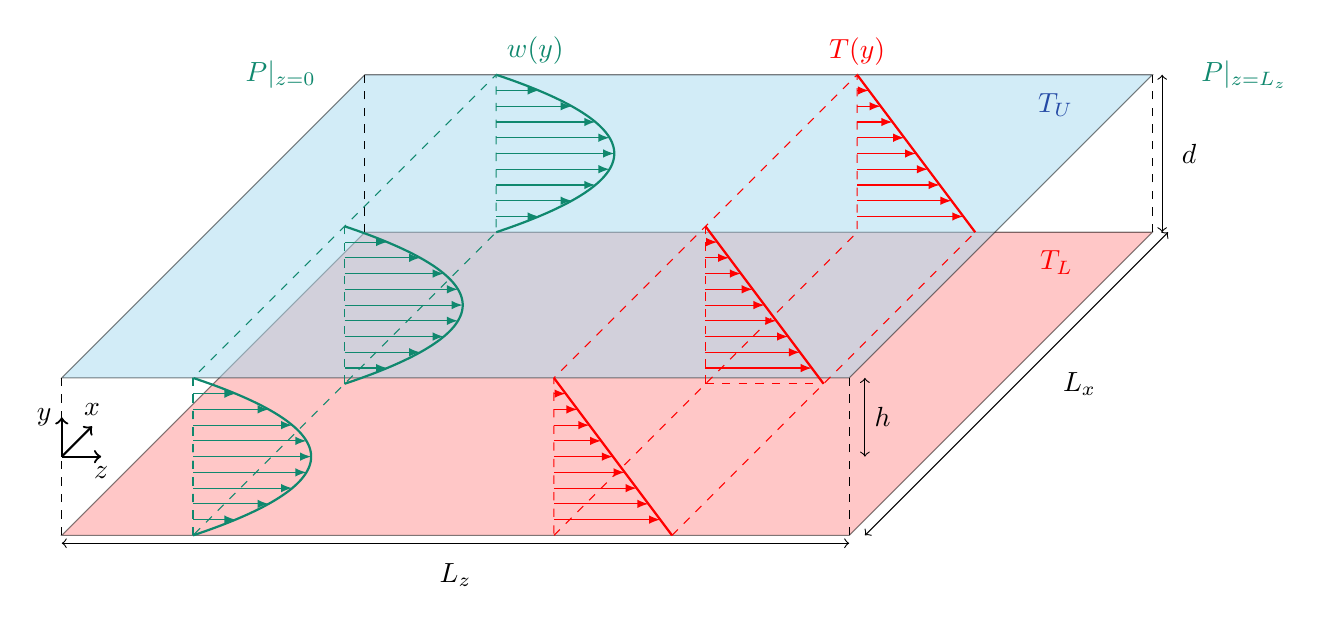
\begin{tikzpicture}
\def\H{1}
\def\W{10}
\def\L{10}

% Draw the bottom plate
\draw [fill=pink!75!red, opacity=0.5] (-\L/2,-\H,0) -- (\L/2,-\H,0) -- (\L/2, -\H, -\W) -- (-\L/2, -\H,-\W) -- cycle;

% Draw the top plate
\draw [fill=SkyBlue!75!white, opacity=0.5] (-\L/2,\H,0) -- (\L/2,\H,0) -- (\L/2, \H, -\W) -- (-\L/2,\H,-\W) -- cycle;

%  % Draw axes
\draw [dashed, thin] (-\L/2, -\H, 0) -- (-\L/2, \H, 0);
\draw [dashed, thin] (\L/2, -\H, 0) -- (\L/2, \H, 0);
\draw [dashed, thin] (\L/2, -\H, -\W) -- (\L/2, \H, -\W);
\draw [dashed, thin] (-\L/2, -\H, -\W) -- (-\L/2, \H, -\W);
%\draw [dashed, thin] (-1,0, 0) --++ (\L,0,0) --++ (0,0,-\W) --++ (-\L,0,0) -- cycle;
%  % \draw [thin, dashed] (-1,0) -- (6,0);

% Add dimensions
% L_x
\draw [<->] (-\L/2,-1.1*\H, 0) -- (\L/2,-1.1*\H,0);
\node[centered] at (0,-1.5*\H,0) {$L_z$};
 
% L_z
\draw [<->] (\L/2*1.025, -\H, -\W) -- (\L/2*1.025, \H,-\W);
\node[right] at (\L/2*1.05,0.0,-\W) {$d$};

% d
\draw [<->] (\L/2*1.04, -\H) -- (\L/2*1.04,-\H,-\W);
\node[centered] at (\L/2*1.2,-\H,-\W/2) {$L_x$};

% h
\draw [<->] (\L/2*1.04, 0, 0) -- (\L/2*1.04, \H, 0);
\node[right] at (\L/2*1.04,\H/2,0) {$h$};

% P
\node[left] at (-\L/2*1.1, \H, -\W) {\textcolor{PineGreen}{$P|_{z=0}$}};
\node[right] at (\L/2*1.1, \H, -\W) {\textcolor{PineGreen}{$P|_{z=L_z}$}};

% T
\node[left] at (\L/2*0.9, \H, -\W*0.9) {\textcolor{cyan!20!blue}{$T_U$}};
\node[left] at (\L/2*0.9, -\H, -\W*0.9) {\textcolor{red}{$T_L$}};

% Draw labels
\draw[->, thick] (-\L/2, 0, 0) -- (-\L/2,\H/2,0) node[left] {$y$};
\draw[->, thick] (-\L/2, 0, 0) -- (-\L/2+\H/2,0,0) node [below] {$z$};
\draw[->, thick] (-\L/2, 0, 0) -- (-\L/2,0,-\H) node[above] {$x$};

% Draw the velocity profile
\draw[PineGreen,thick,domain=-1:1,samples=200,smooth] plot ({(1-\x*\x)*1.5-\L/3}, \x) node[above right] {};
\draw[PineGreen,thick,domain=-1:1,samples=200,smooth] plot ({(1-\x*\x)*1.5-\L/3}, \x, -\W/2) node[above right] {};
\draw[PineGreen,thick,domain=-1:1,samples=200,smooth] plot ({(1-\x*\x)*1.5-\L/3}, \x, -\W) node[above right] {$w(y)$};
\draw[-,PineGreen,dashed] (-\L/3,-\H) -- (-\L/3,\H);
\draw[-,PineGreen,dashed] (-\L/3,-\H, -\W/2) -- (-\L/3,\H, -\W/2);
\draw[-,PineGreen,dashed] (-\L/3,-\H,0) -- (-\L/3,\H,0) -- (-\L/3,\H,-\W) -- (-\L/3,-\H,-\W) -- cycle;

\foreach \y in {-0.8,-0.6,...,0.8} {
    \draw[-latex,PineGreen] (-\L/3,\y, 0) -- ({(1-\y*\y)*1.5-\L/3},\y,0);
    \draw[-latex,PineGreen] (-\L/3,\y, -\W/2) -- ({(1-\y*\y)*1.5-\L/3},\y, -\W/2);
    \draw[-latex,PineGreen] (-\L/3,\y, -\W) -- ({(1-\y*\y)*1.5-\L/3},\y,-\W);
}

% Draw the temperature profile
\draw[red,thick,domain=-\H:\H,samples=200,smooth] plot ({(1/2*(1-\x)*1.5+\L/8)}, \x);
\draw[red,thick,domain=-\H:\H,samples=200,smooth] plot ({(1/2*(1-\x)*1.5+\L/8)}, \x, -\W/2);
\draw[red,thick,domain=-\H:\H,samples=200,smooth] plot ({(1/2*(1-\x)*1.5+\L/8)}, \x, -\W);
\draw[-,red,dashed] (\L/8,-\H,-\W/2) -- (\L/8,\H,-\W/2);
\draw[-,red,dashed] (\L/8,-\H,-\W/2) -- (\L/8 + 1.5,-\H,-\W/2);
\draw[-,red,dashed] (\L/8 +1.5,-\H,0) -- (\L/8 + 1.5,-\H,-\W);
\draw[-,red,dashed] (\L/8,-\H,0) -- (\L/8,-\H,-\W) -- (\L/8,\H, -\W) -- (\L/8,\H,0) -- cycle;
% % 
\foreach \y in {-0.8,-0.6,...,0.8} {
   \draw[-latex,red] (\L/8,\y) -- ({\L/8+(1/2*(1-\y)*1.5},\y);
   \draw[-latex,red] (\L/8,\y, -\W/2) -- ({\L/8+(1/2*(1-\y)*1.5},\y, -\W/2);
   \draw[-latex,red] (\L/8,\y, -\W) -- ({\L/8+(1/2*(1-\y)*1.5},\y, -\W);
}
% Add labels
\node[above,red] at (\L/8,1,-\W) {$T(y)$};
\end{tikzpicture}
\label{fig:rbpconfiguration}
\caption{The Rayleigh-B\'{e}nard Poiseuille (RBP) flow configuration.}
\end{figure}
